%!Tex Program = xelatex
\documentclass[a4paper]{ctexart} % 使用 ctexart 支持中文
\usepackage{amsmath} % 数学公式支持
\usepackage{amsfonts} % 数学符号支持
\usepackage{amssymb} % 数学符号支持
\usepackage{graphicx} % 图片支持
\usepackage{subcaption} % 子图支持
\usepackage{fontspec} % 字体支持

% 定义拉普拉斯算子
\newcommand{\laplace}{\ensuremath{\Delta}}

% 文档信息
\title{Project1 Report}
\author{匿}
\date{2024年3月14日}

\begin{document}
\maketitle

\pagestyle{empty}

\section{问题描述}
本项目的目标是在给定区域 $\Omega$ 上求解泊松方程 $-\laplace u = f$，其中区域 $\Omega$ 和边界条件由用户指定。具体问题描述如下：

\subsection{区域定义}
用户可以选择以下两种区域之一：
\begin{itemize}
    \item[(a)] 正方形区域 $\Omega = (0, 1)^2$；
    \item[(b)] 区域 $\Omega \setminus D$，其中 $D$ 是一个用户指定的闭合圆盘。圆盘的半径和中心由用户输入，且需满足以下条件：
    \begin{itemize}
        \item $\Omega \setminus D$ 必须是连通的；
        \item 圆盘 $D$ 必须覆盖至少四个方程离散化点；
    \end{itemize}
    为了保持数值上的性质，我们要求用户给出的圆在``数值上''是不与边界有交的，即圆距离区域边界的距离大于 $h$（网格单位长度）。
\end{itemize}

\subsection{边界条件}
用户可以选择以下边界条件之一：
\begin{itemize}
    \item Dirichlet 边界条件；
    \item Neumann 边界条件；
    \item 混合边界条件（部分 Dirichlet，部分 Neumann）。
\end{itemize}

\subsection{问题图示}
求解区域 $\Omega \setminus D$ 的示意图如下。
\begin{figure}[htbp]
    \centering
    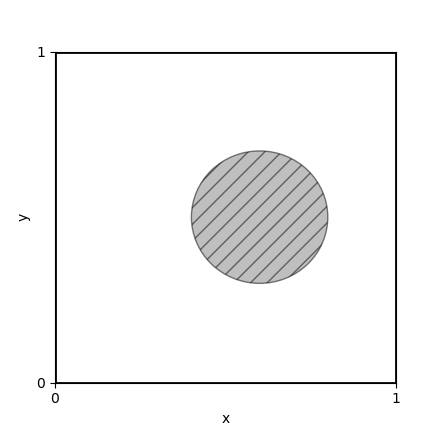
\includegraphics[width=0.2\textwidth]{Figure_1.png} % 确保图片路径正确
    \caption{区域 $\Omega \setminus D$} 
    \label{fig:domain}
\end{figure}

\section{离散实现与理论分析}
\subsection{一般内部格点的离散}
对于一般内部格点的离散，我们采用讲义中 (7.58) 式的二阶中心差分，$\tau_{i,j} = O(h^2)$。

\subsection{对于方形边界的离散}
对于 Dirichlet 边界条件，我们直接给该点按输入的条件赋值即可。

而对于 Neumann 边界，在边界对称地向外取 ghost cell，如下图。我们对边界 $\frac{\partial u}{\partial n}$ 使用中心差商 $\frac{U_R - U_P}{2h}$ 进行近似，截断误差 $\tau = \frac{1}{6}u''' h^2 + O(h^4) = O(h^2)$。
\begin{figure}[htbp]
    \centering
    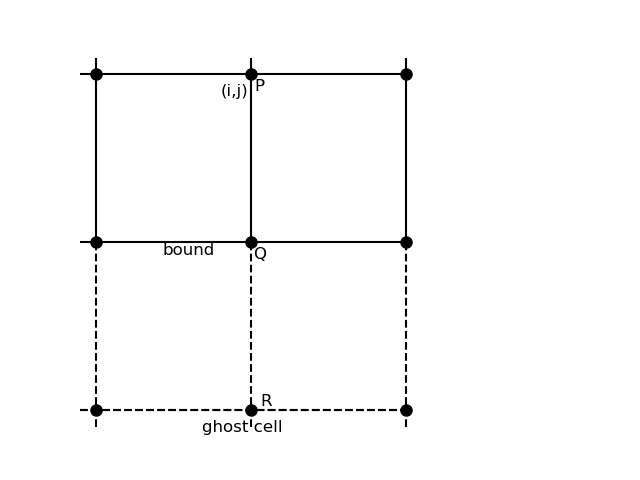
\includegraphics[width=0.6\textwidth]{Figure_2.png} % 确保图片路径正确
    \caption{方形 Neumann 边界} 
    \label{fig:neumann_boundary}
\end{figure}

\subsection{对于圆形内部边界的离散}
对于 Dirichlet 边界条件，采用讲义中 (7.88) 式的方法，对一个待离散的点 $(i,j)$，其不在圆内（否则置 0），对一个圆弧截它的邻居（上下左右四点），只可能截掉其中一个或者两个相邻格点。
故分方向对这个点 $(i,j)$ 应用 (7.88) 即可，在理论作业中已经证明此处截断误差为 $O(h)$。
\begin{figure}[htbp]
    \centering
    \begin{subfigure}[b]{0.45\textwidth}
        \centering
        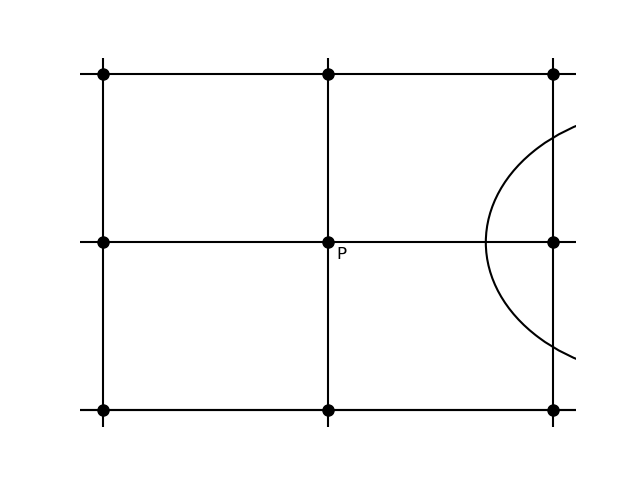
\includegraphics[width=\textwidth]{Figure_3.png}
        \caption{截取一个点}
        \label{fig:image1}
    \end{subfigure}
    \hfill
    \begin{subfigure}[b]{0.45\textwidth}
        \centering
        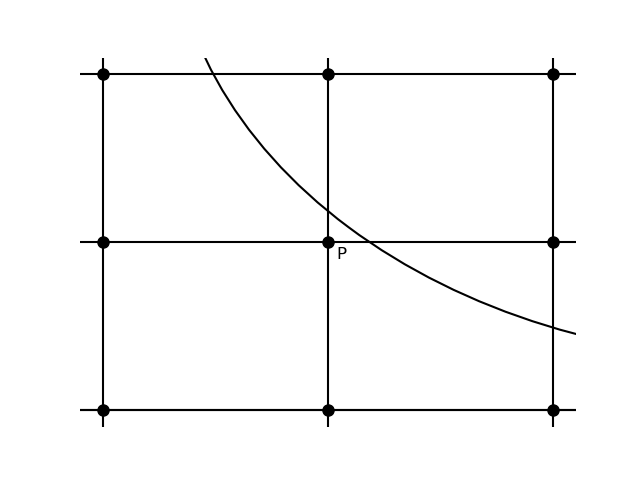
\includegraphics[width=\textwidth]{Figure_4.png}
        \caption{截取两个点}
        \label{fig:image2}
    \end{subfigure}
    \caption{Dirichlet 边界处理}
    \label{fig:dirichlet_boundary}
\end{figure}

而对于 Neumann 边界条件，对于上述 $(i,j)$，我们由于要处理法向导数信息，做拟合时总是需要圆心和圆边界两个点。
对上面两种分类在操作层面可能过于麻烦，希望有一个对 $(i,j)$ 的统一处理方式，设 $(i,j)$ 这个点为点 $P$，我们由圆心向 $P$ 点做射线。
这条射线交圆边界于点 $Q$，交 $P$ 的邻居``田''字区域于点 $T$。

\begin{figure}[htbp]
    \centering
    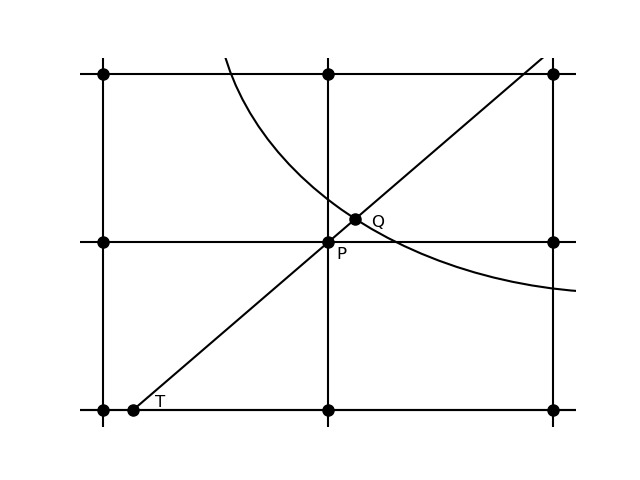
\includegraphics[width=0.6\textwidth]{Figure_5.png} % 确保图片路径正确
    \caption{Neumann 边界条件辅助线} 
    \label{fig:neumann_auxiliary}
\end{figure}

这里我用
\[
\frac{U_T - U_P}{PT} = \frac{\partial u}{\partial n}(Q),
\]
其中 $U_T$ 由 $U_R$ 和 $U_S$ 插值得到，即
\[
U_T = \frac{TS}{h} \cdot U_R + \frac{RT}{h} \cdot U_S.
\]

这样就得到了一个对 Neumann 边界的近似处理，这里的 $\tau = O(h)$。

\section{程序设计逻辑}
\subsection{问题域与边界条件定义}
\textbf{ProblemDomain 类} 用于初始化问题所有的几何域和边界条件，支持两种类型的域：
\begin{itemize}
    \item \textbf{默认方形区域} 和 \textbf{带有圆形区域的区域}。
    \item 边界条件类型支持 \textbf{Dirichlet}、\textbf{Neumann} 和 \textbf{混合边界条件}，通过 \texttt{BCType} 和 \texttt{MixedType} 枚举类型指定。
    \item 通过 \texttt{setSquareBoundaryCondition} 和 \texttt{setCircleBoundaryCondition} 方法设置方形和圆形边界的边界条件函数。
    \item 提供几何判断功能，包括判断点是否在圆形区域内的 \texttt{isPointInsideCircle}，以及计算射线与圆形或方形区域交点的 \texttt{getRayCircleIntersection} 和 \texttt{getRaySquareIntersection}。
\end{itemize}

\textbf{BVPSolver 类} 负责构建线性方程组并求解，依赖于 \texttt{ProblemDomain} 类获取问题域和边界条件信息：
\begin{itemize}
    \item 初始化矩阵 \texttt{A} 和向量 \texttt{F}，分别存储线性系统的系数矩阵和右端向量。
    \item 根据边界条件类型（Dirichlet、Neumann 或混合边界条件）构建线性方程组，处理边界条件。
\end{itemize}

\section{收敛性测试}
对内部格点和方形边界误差取对数的线性拟合如下，效果显示基本符合理论预期。
\clearpage
\begin{figure}[htbp]
    \centering
    \begin{subfigure}[b]{0.45\textwidth}
        \centering
        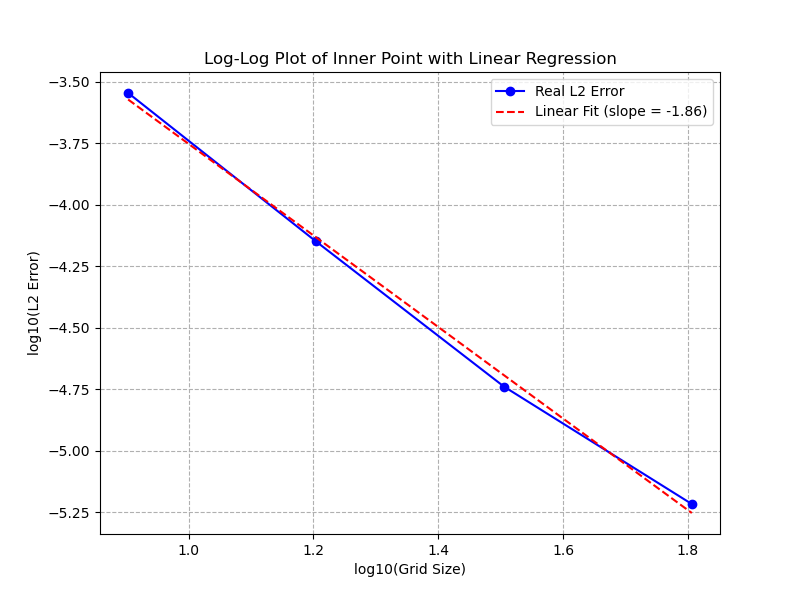
\includegraphics[width=\textwidth]{error_analysis_test/Inner_Point.png}
        \caption{一般内部格点}
        \label{fig:inner_point}
    \end{subfigure}
    \hfill
    \begin{subfigure}[b]{0.45\textwidth}
        \centering
        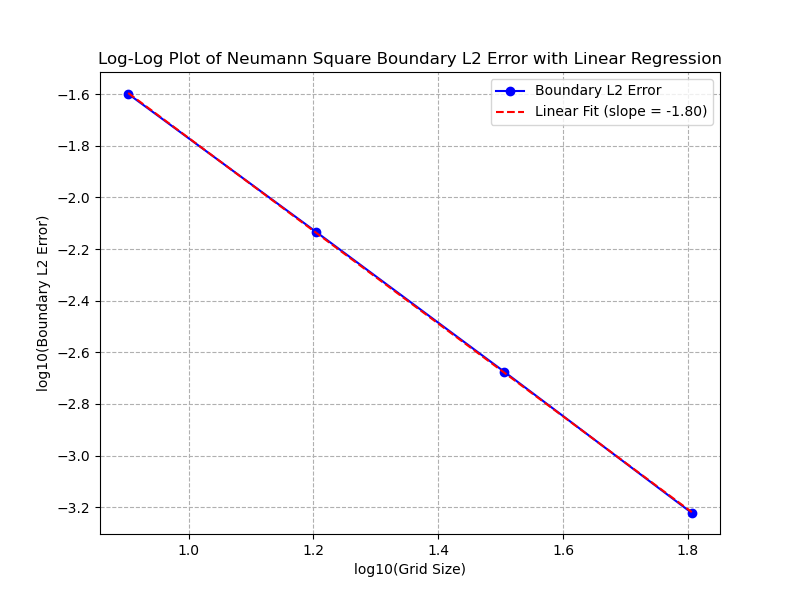
\includegraphics[width=\textwidth]{error_analysis_test/Neumann_Square.png}
        \caption{方形 Neumann 边界}
        \label{fig:neumann_square}
    \end{subfigure}
    \caption{误差测试}
    \label{fig:error_analysis}
\end{figure}

对圆形边界的测试如下：
\begin{figure}[htbp]
    \centering
    \begin{subfigure}[b]{0.45\textwidth}
        \centering
        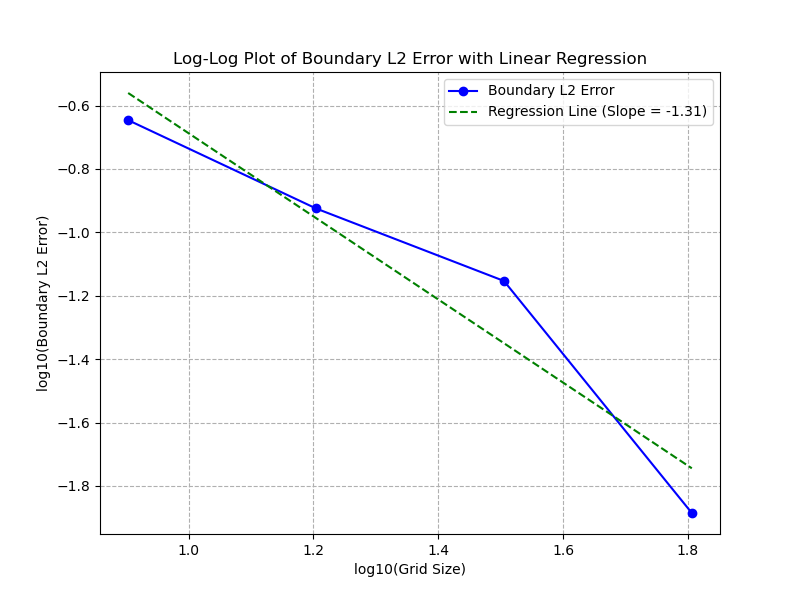
\includegraphics[width=\textwidth]{error_analysis_test/Circular_ND.png}
        \caption{圆形 Dirichlet 边界}
        \label{fig:circular_nd}
    \end{subfigure}
    \hfill
    \begin{subfigure}[b]{0.45\textwidth}
        \centering
        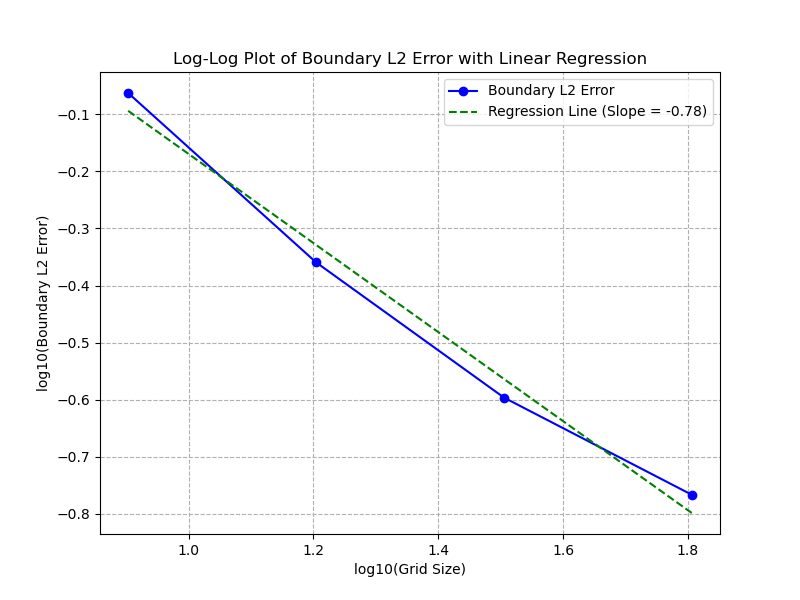
\includegraphics[width=\textwidth]{error_analysis_test/Circular_DN.png}
        \caption{圆形 Dirichlet 边界}
        \label{fig:circular_dn}
    \end{subfigure}
    \caption{误差测试}
    \label{fig:circular_error_analysis}
\end{figure}

\section{结果可视化}
为了便于查看求解效果，我将数值解按几何相对位置存储并且输出为热力图。关于各种格点大小、各种边界组合的测试可以在我的项目目录下 \texttt{make plot} 进入 \texttt{plot} 目录中查看。
此外，我选择了 $u_1 = x + y$ 和 $u_2 = \exp(x + y)$ 进行测试，以下是对效果的举例展示：
\clearpage
\begin{figure}[htbp]
    \centering
    \begin{subfigure}[b]{0.35\textwidth}
        \centering
        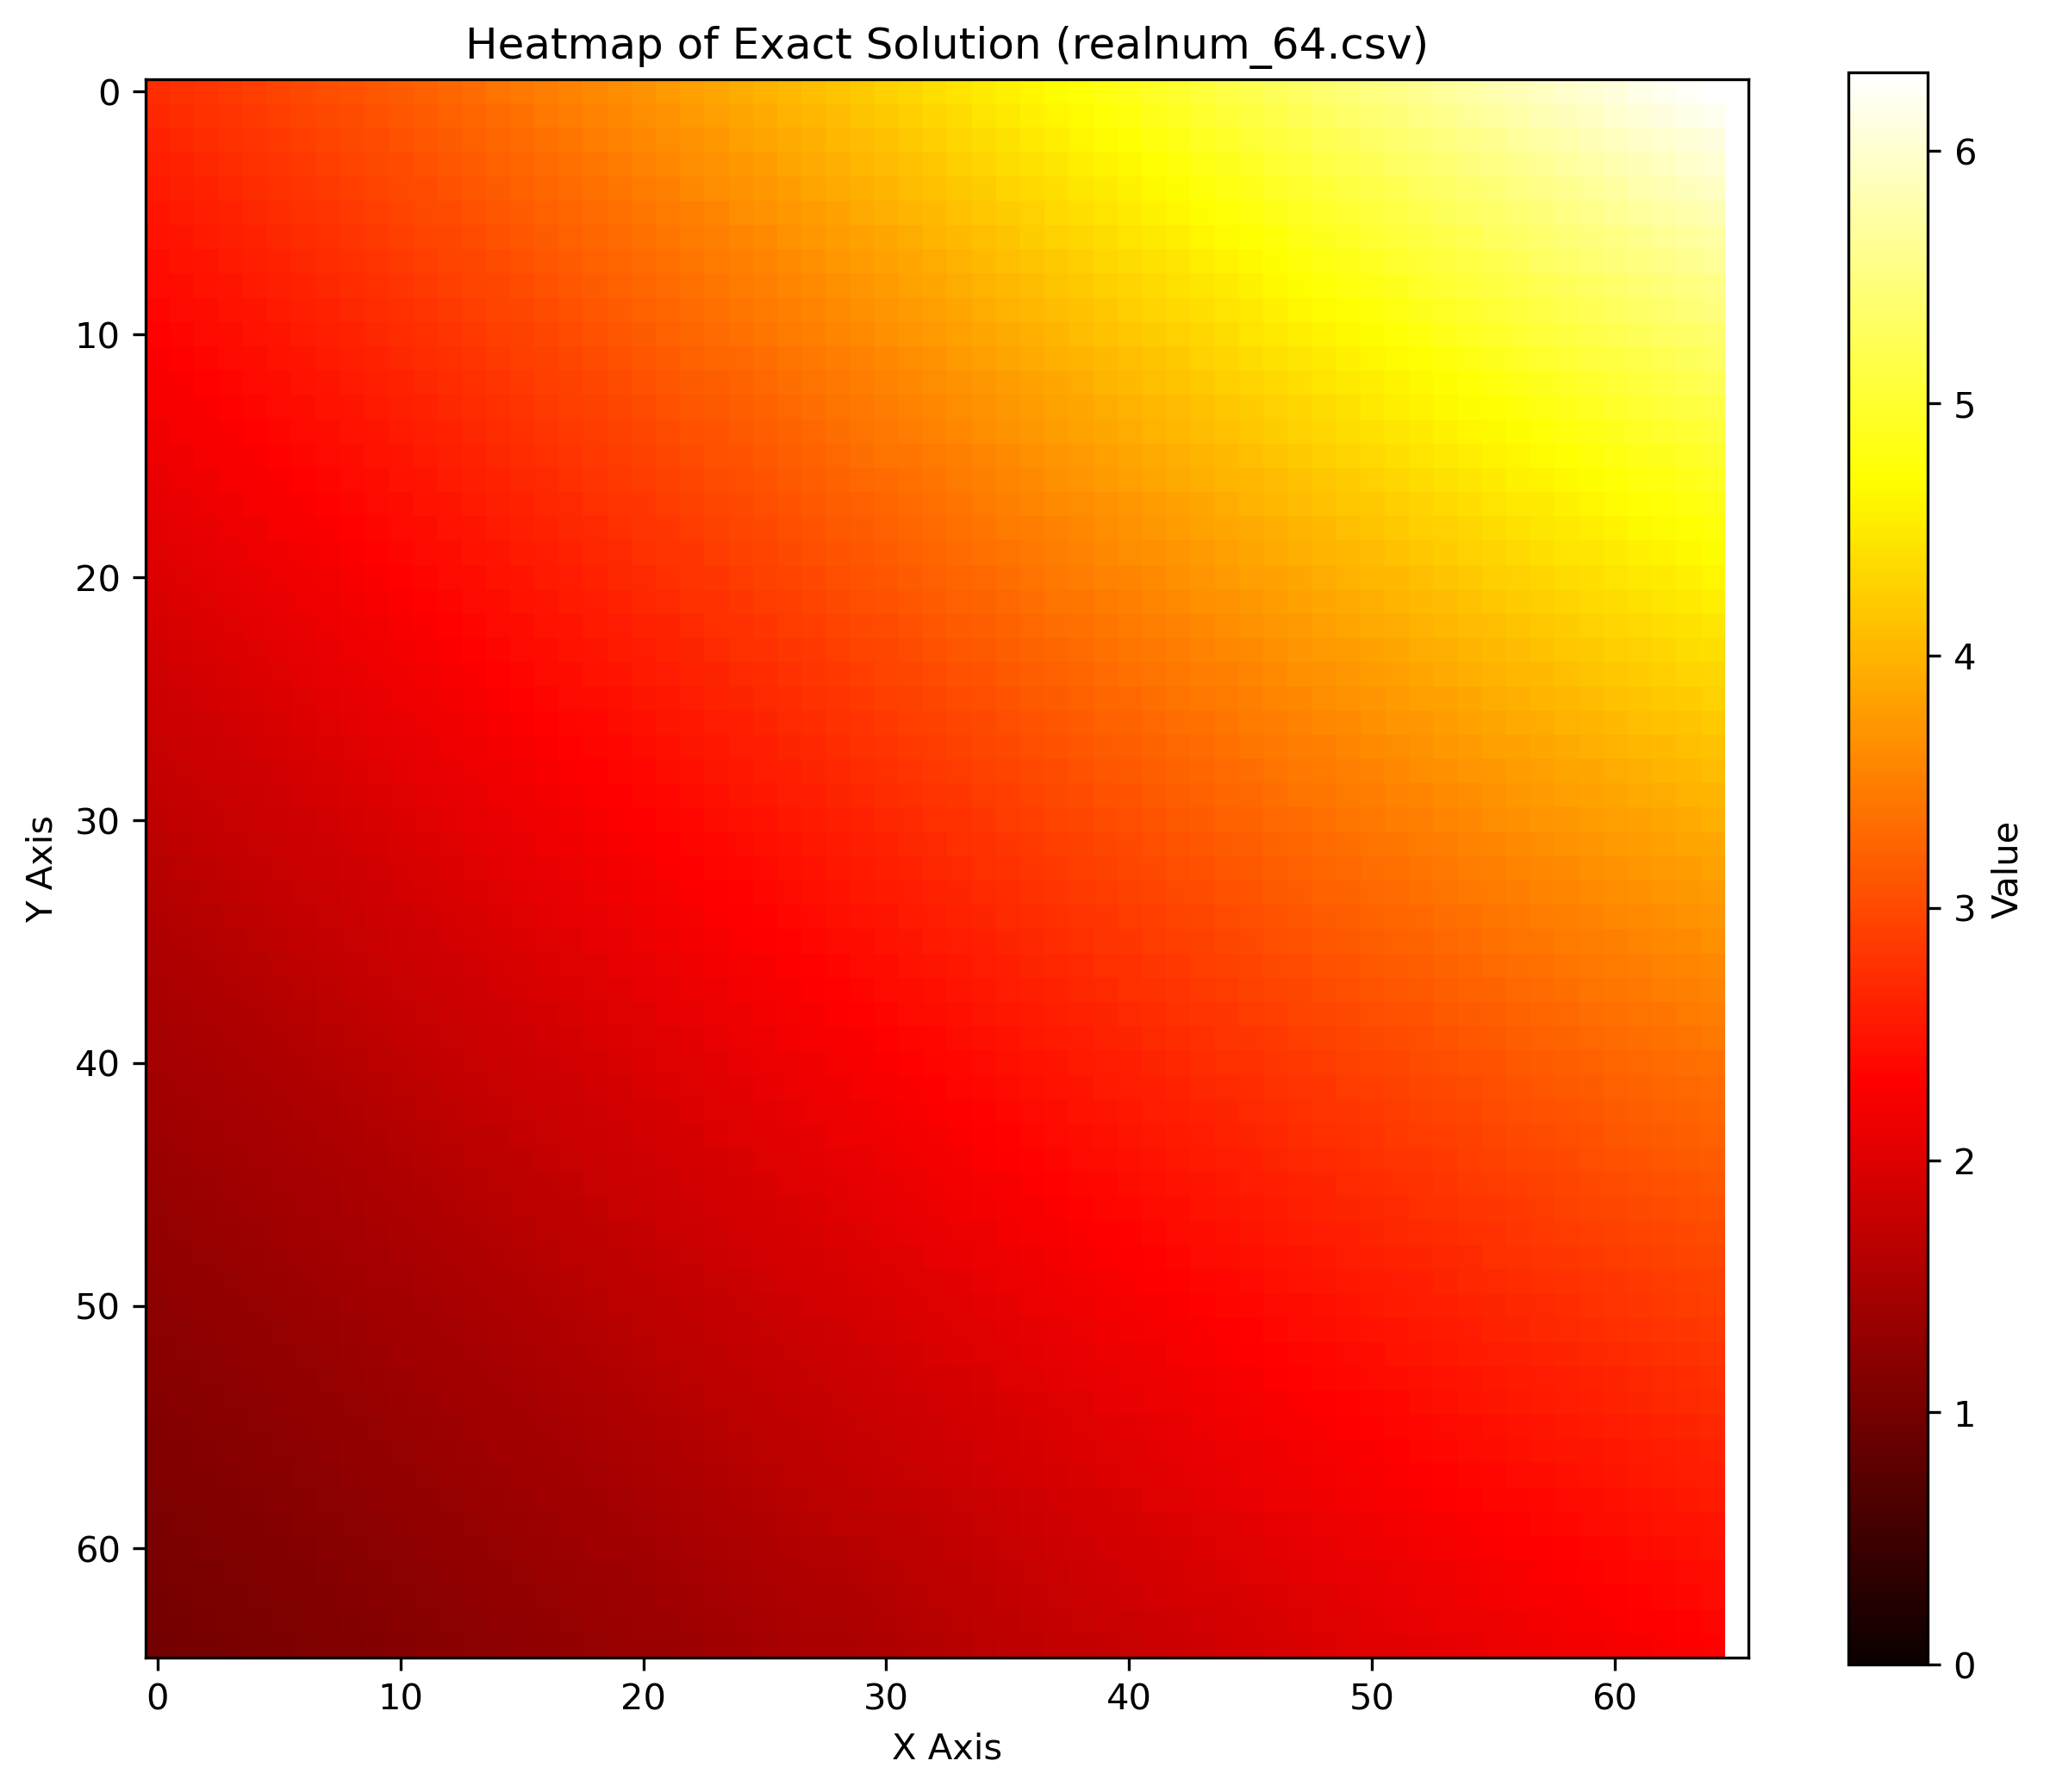
\includegraphics[width=\textwidth]{Figure_6.png}
        \caption{真解}
        \label{fig:true_solution}
    \end{subfigure}
    \hfill
    \begin{subfigure}[b]{0.35\textwidth}
        \centering
        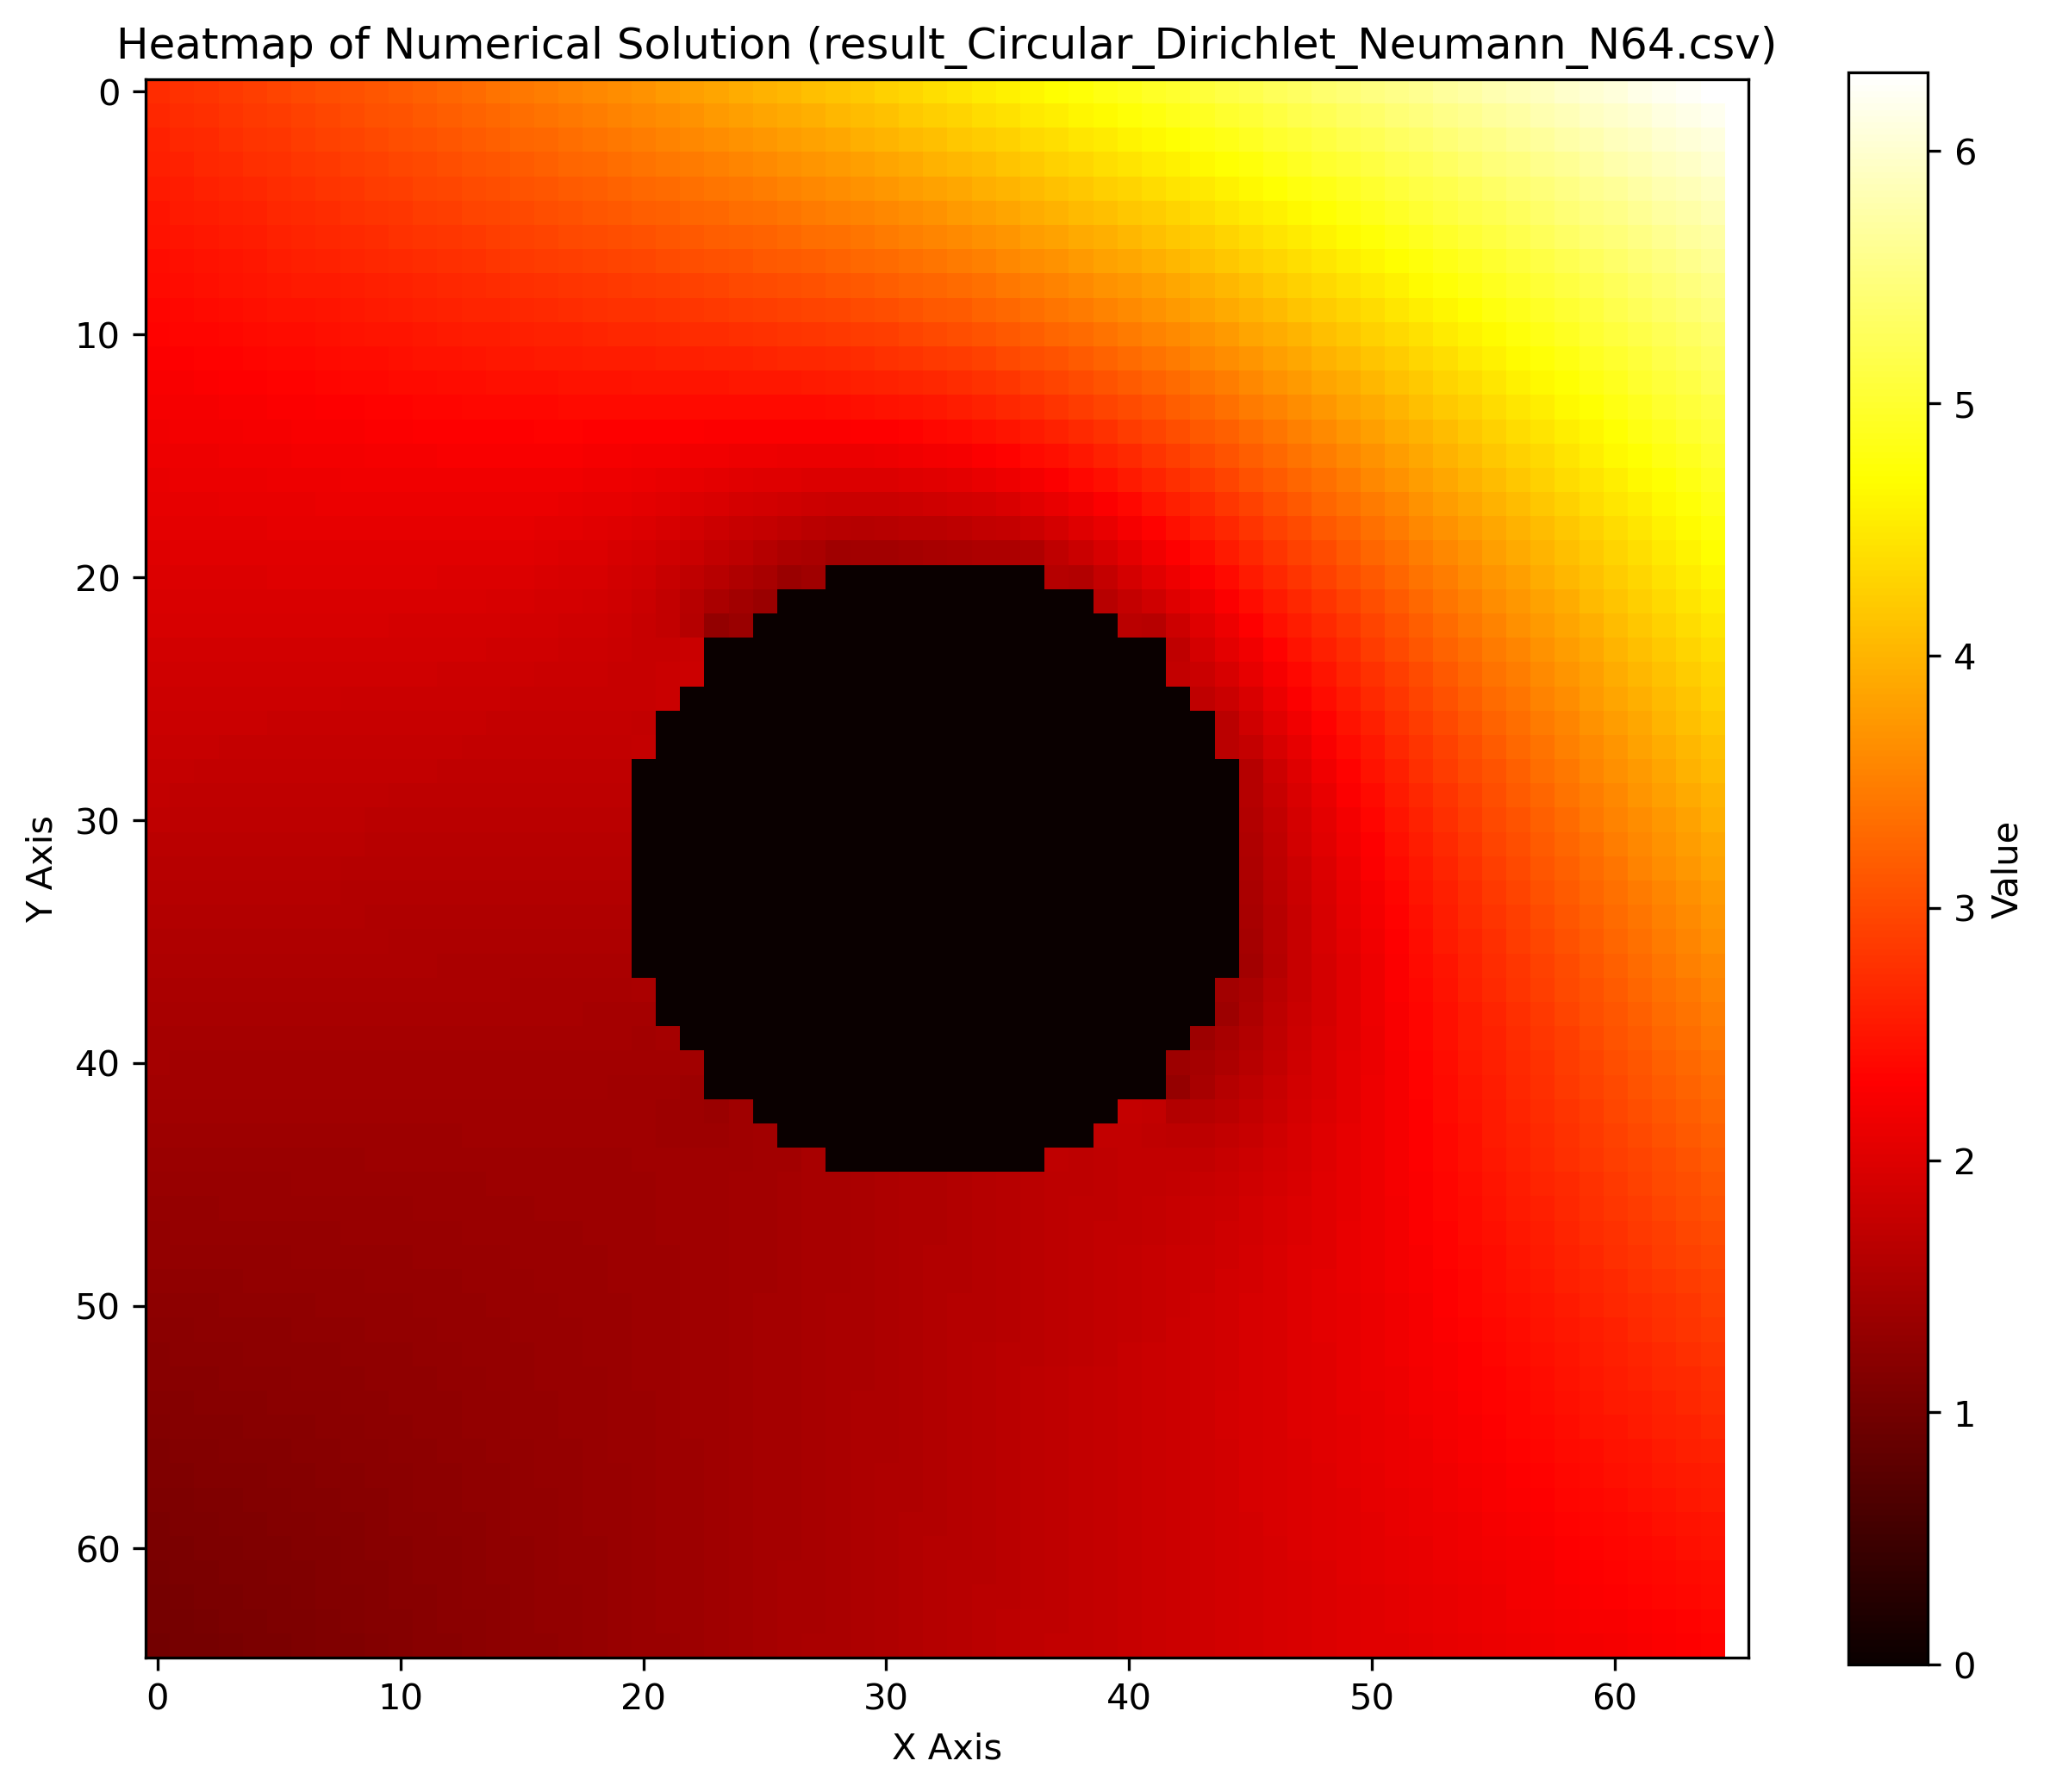
\includegraphics[width=\textwidth]{Figure_7.png}
        \caption{Dirichlet + 圆形 Neumann}
        \label{fig:dirichlet_neumann}
    \end{subfigure}
    \begin{subfigure}[b]{0.35\textwidth}
        \centering
        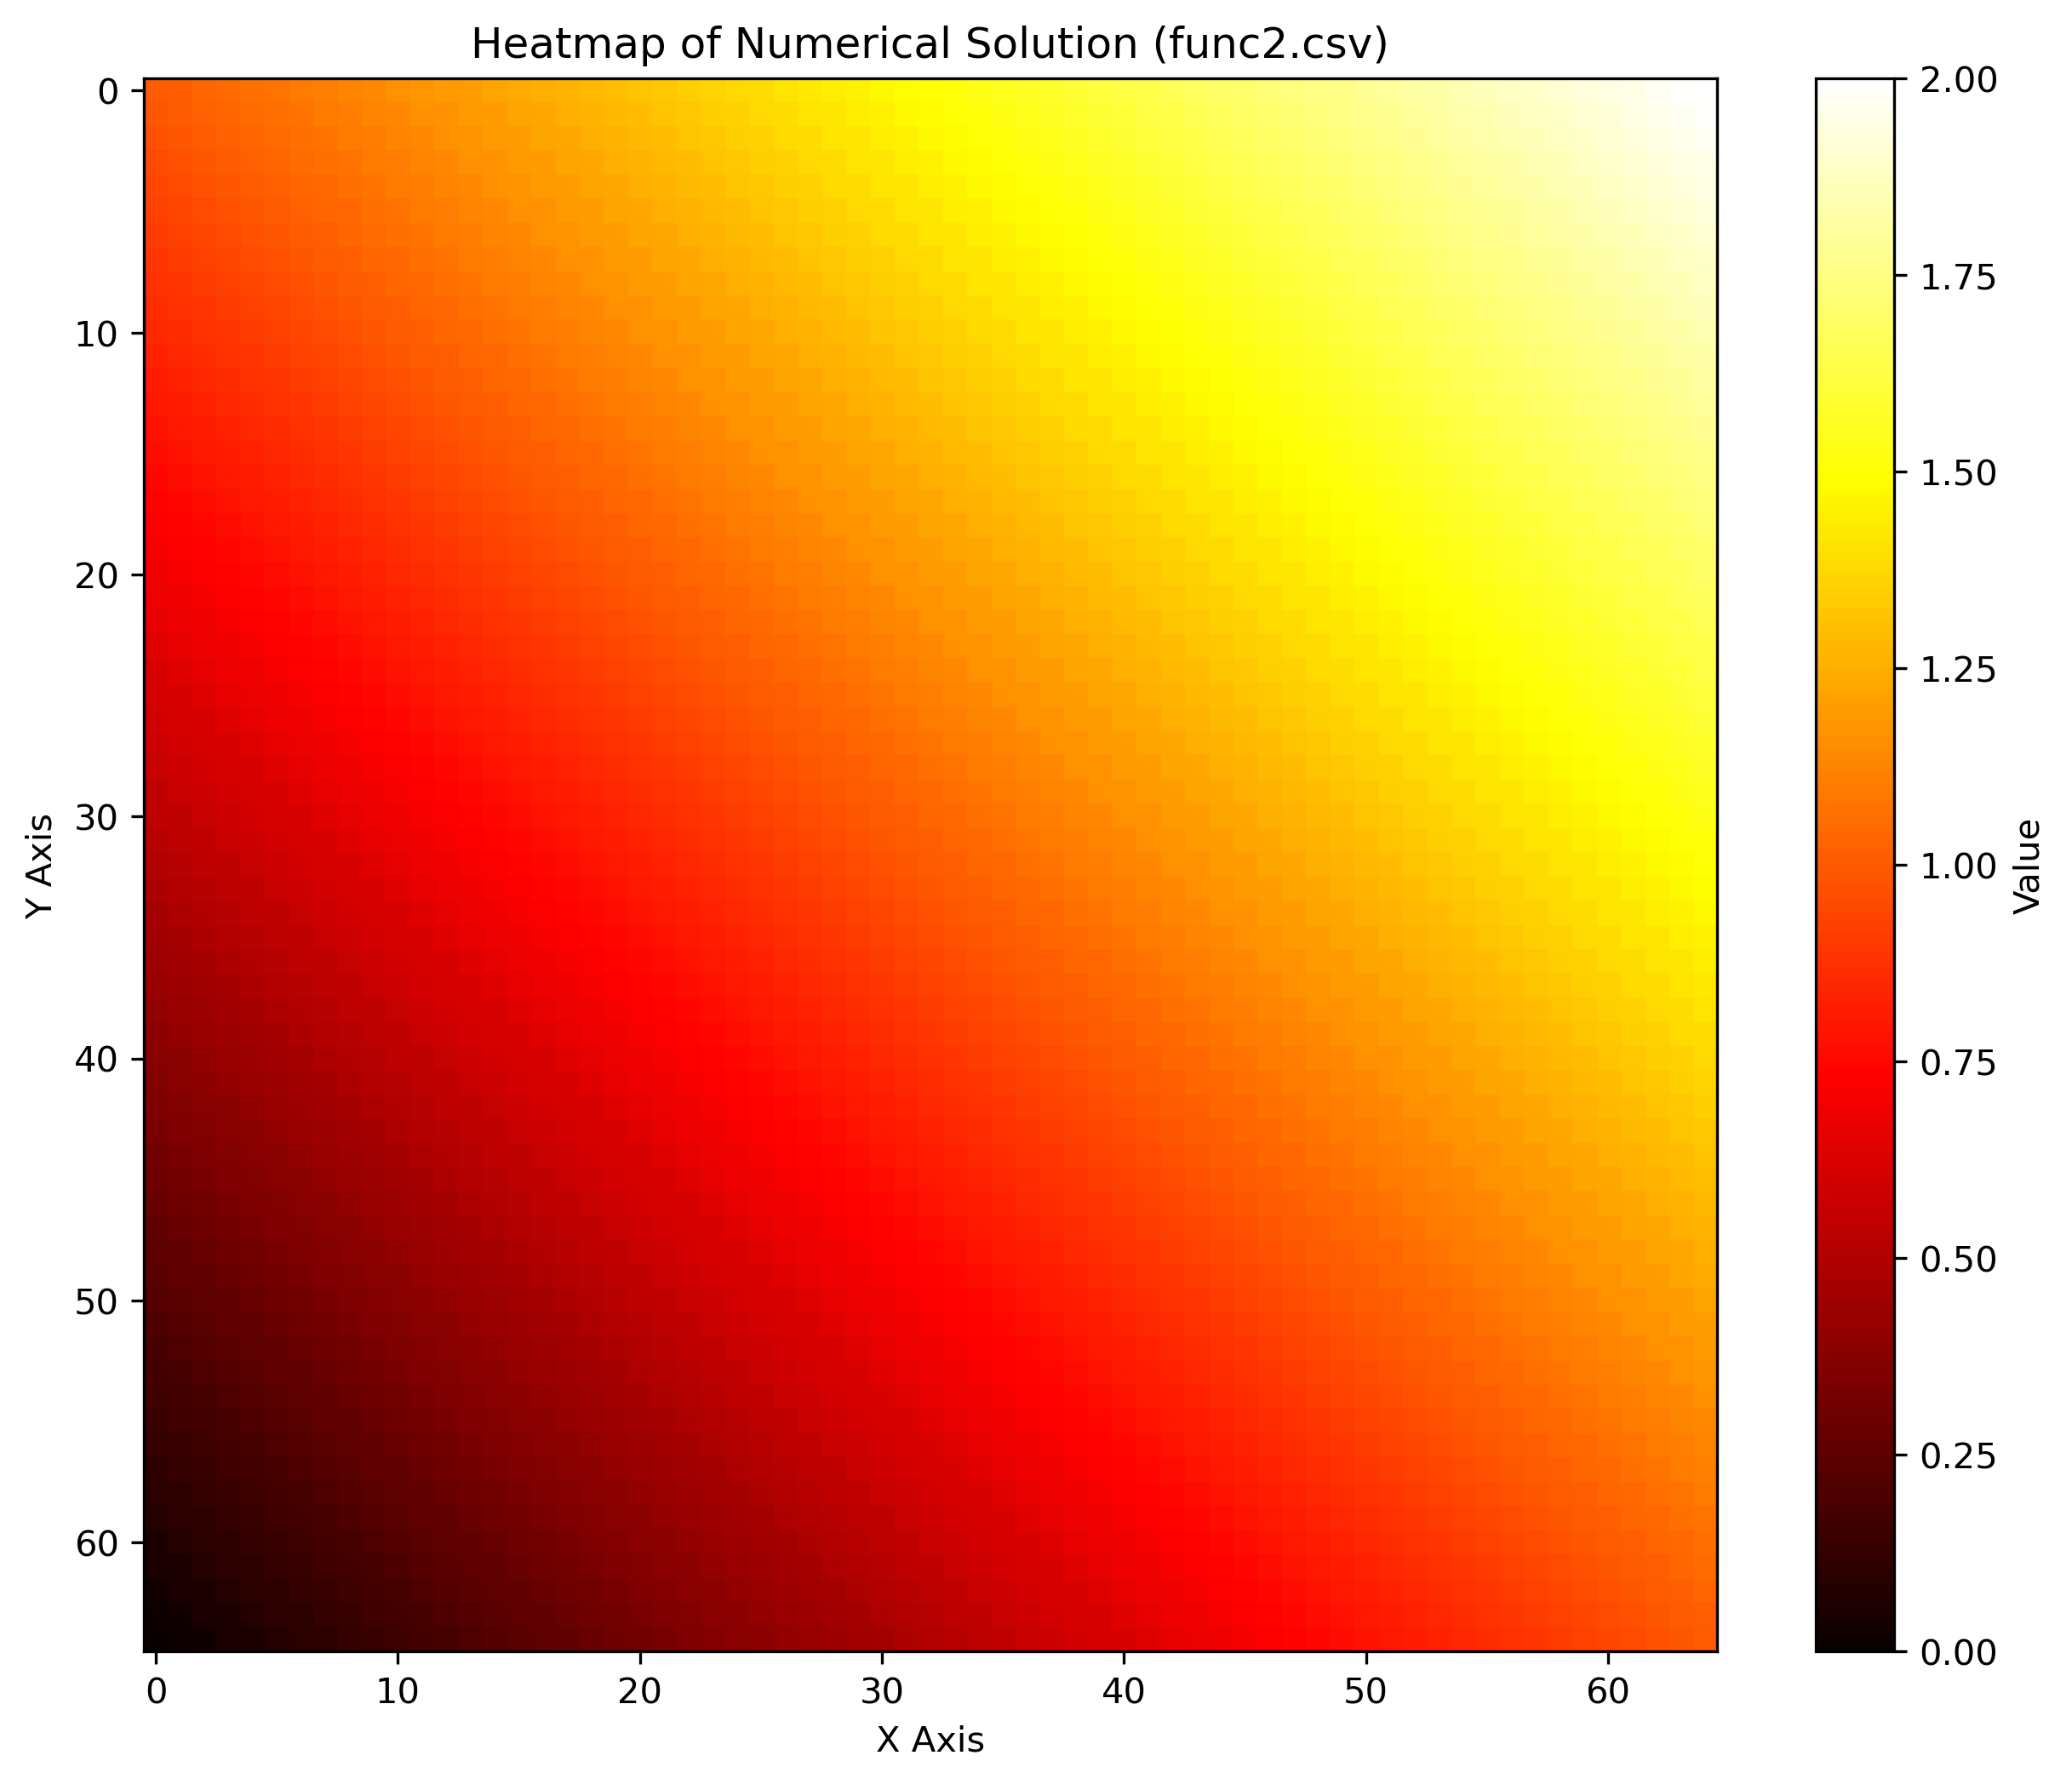
\includegraphics[width=\textwidth]{func2.png}
        \caption{$u = x + y$}
        \label{fig:u_linear}
    \end{subfigure}
    \hfill
    \begin{subfigure}[b]{0.35\textwidth}
        \centering
        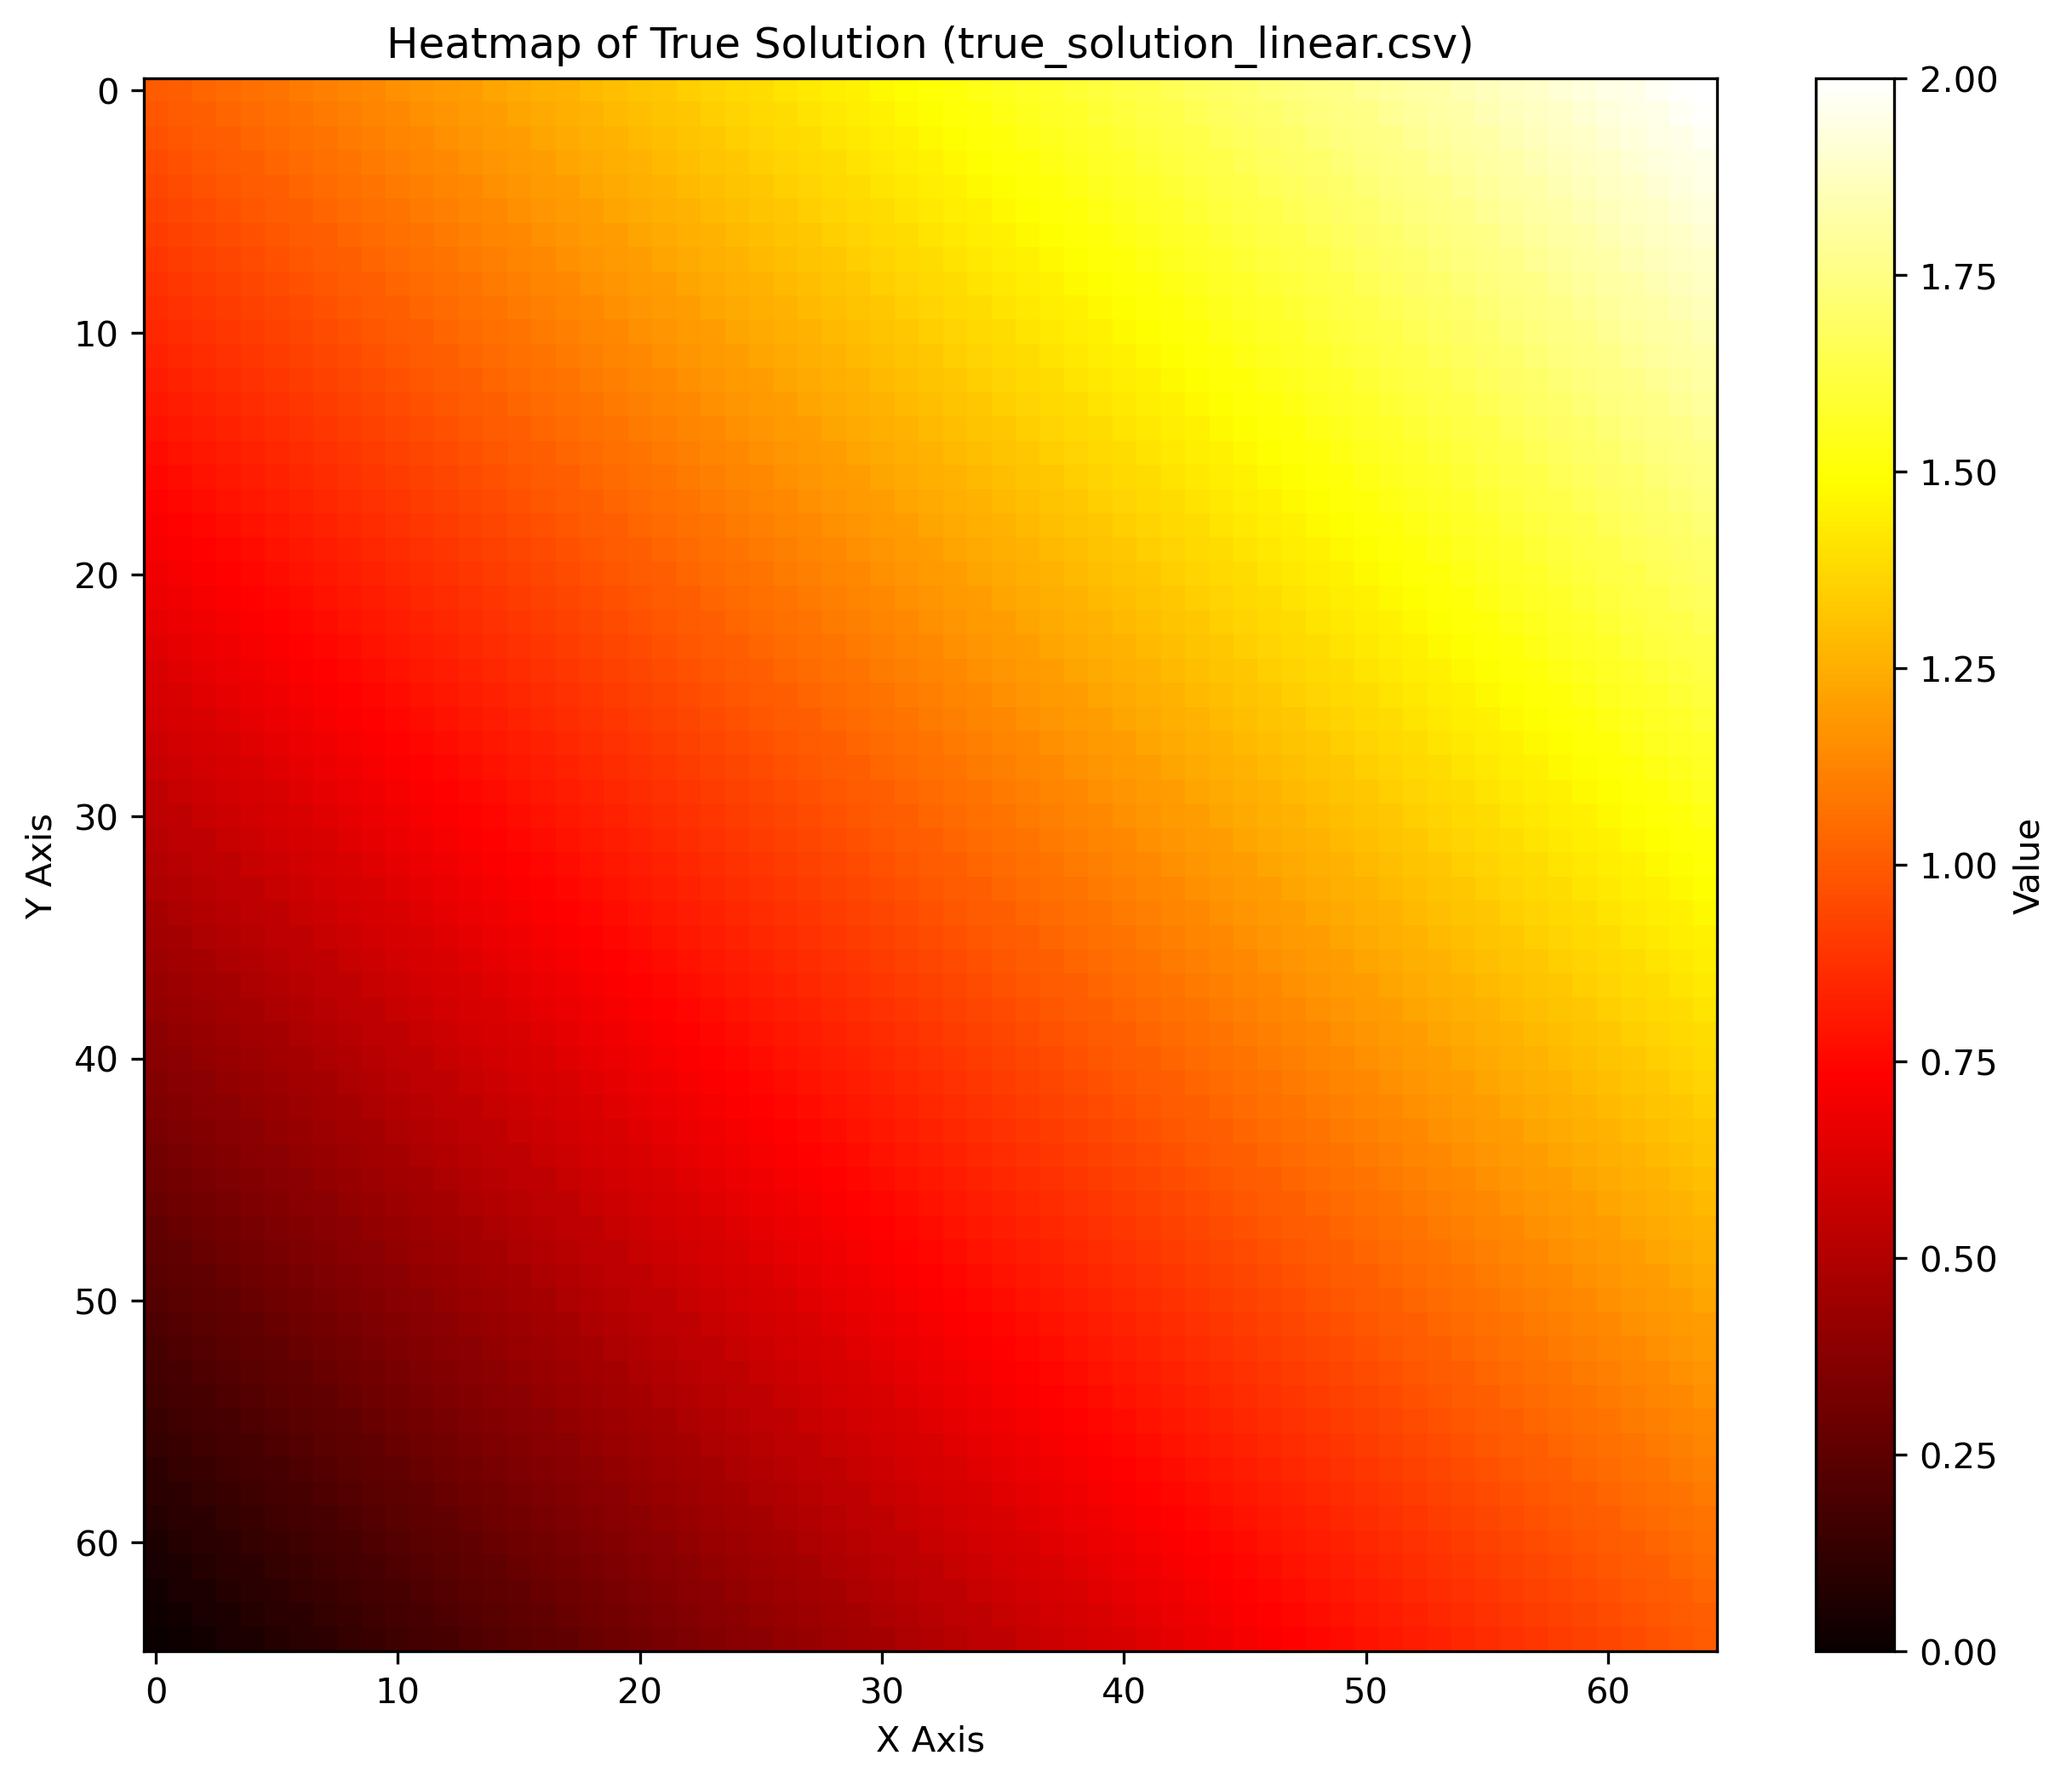
\includegraphics[width=\textwidth]{error_analysis_test/true_solution_linear.png}
        \caption{对应真解}
        \label{fig:true_solution_linear}
    \end{subfigure}
    \begin{subfigure}[b]{0.35\textwidth}
        \centering
        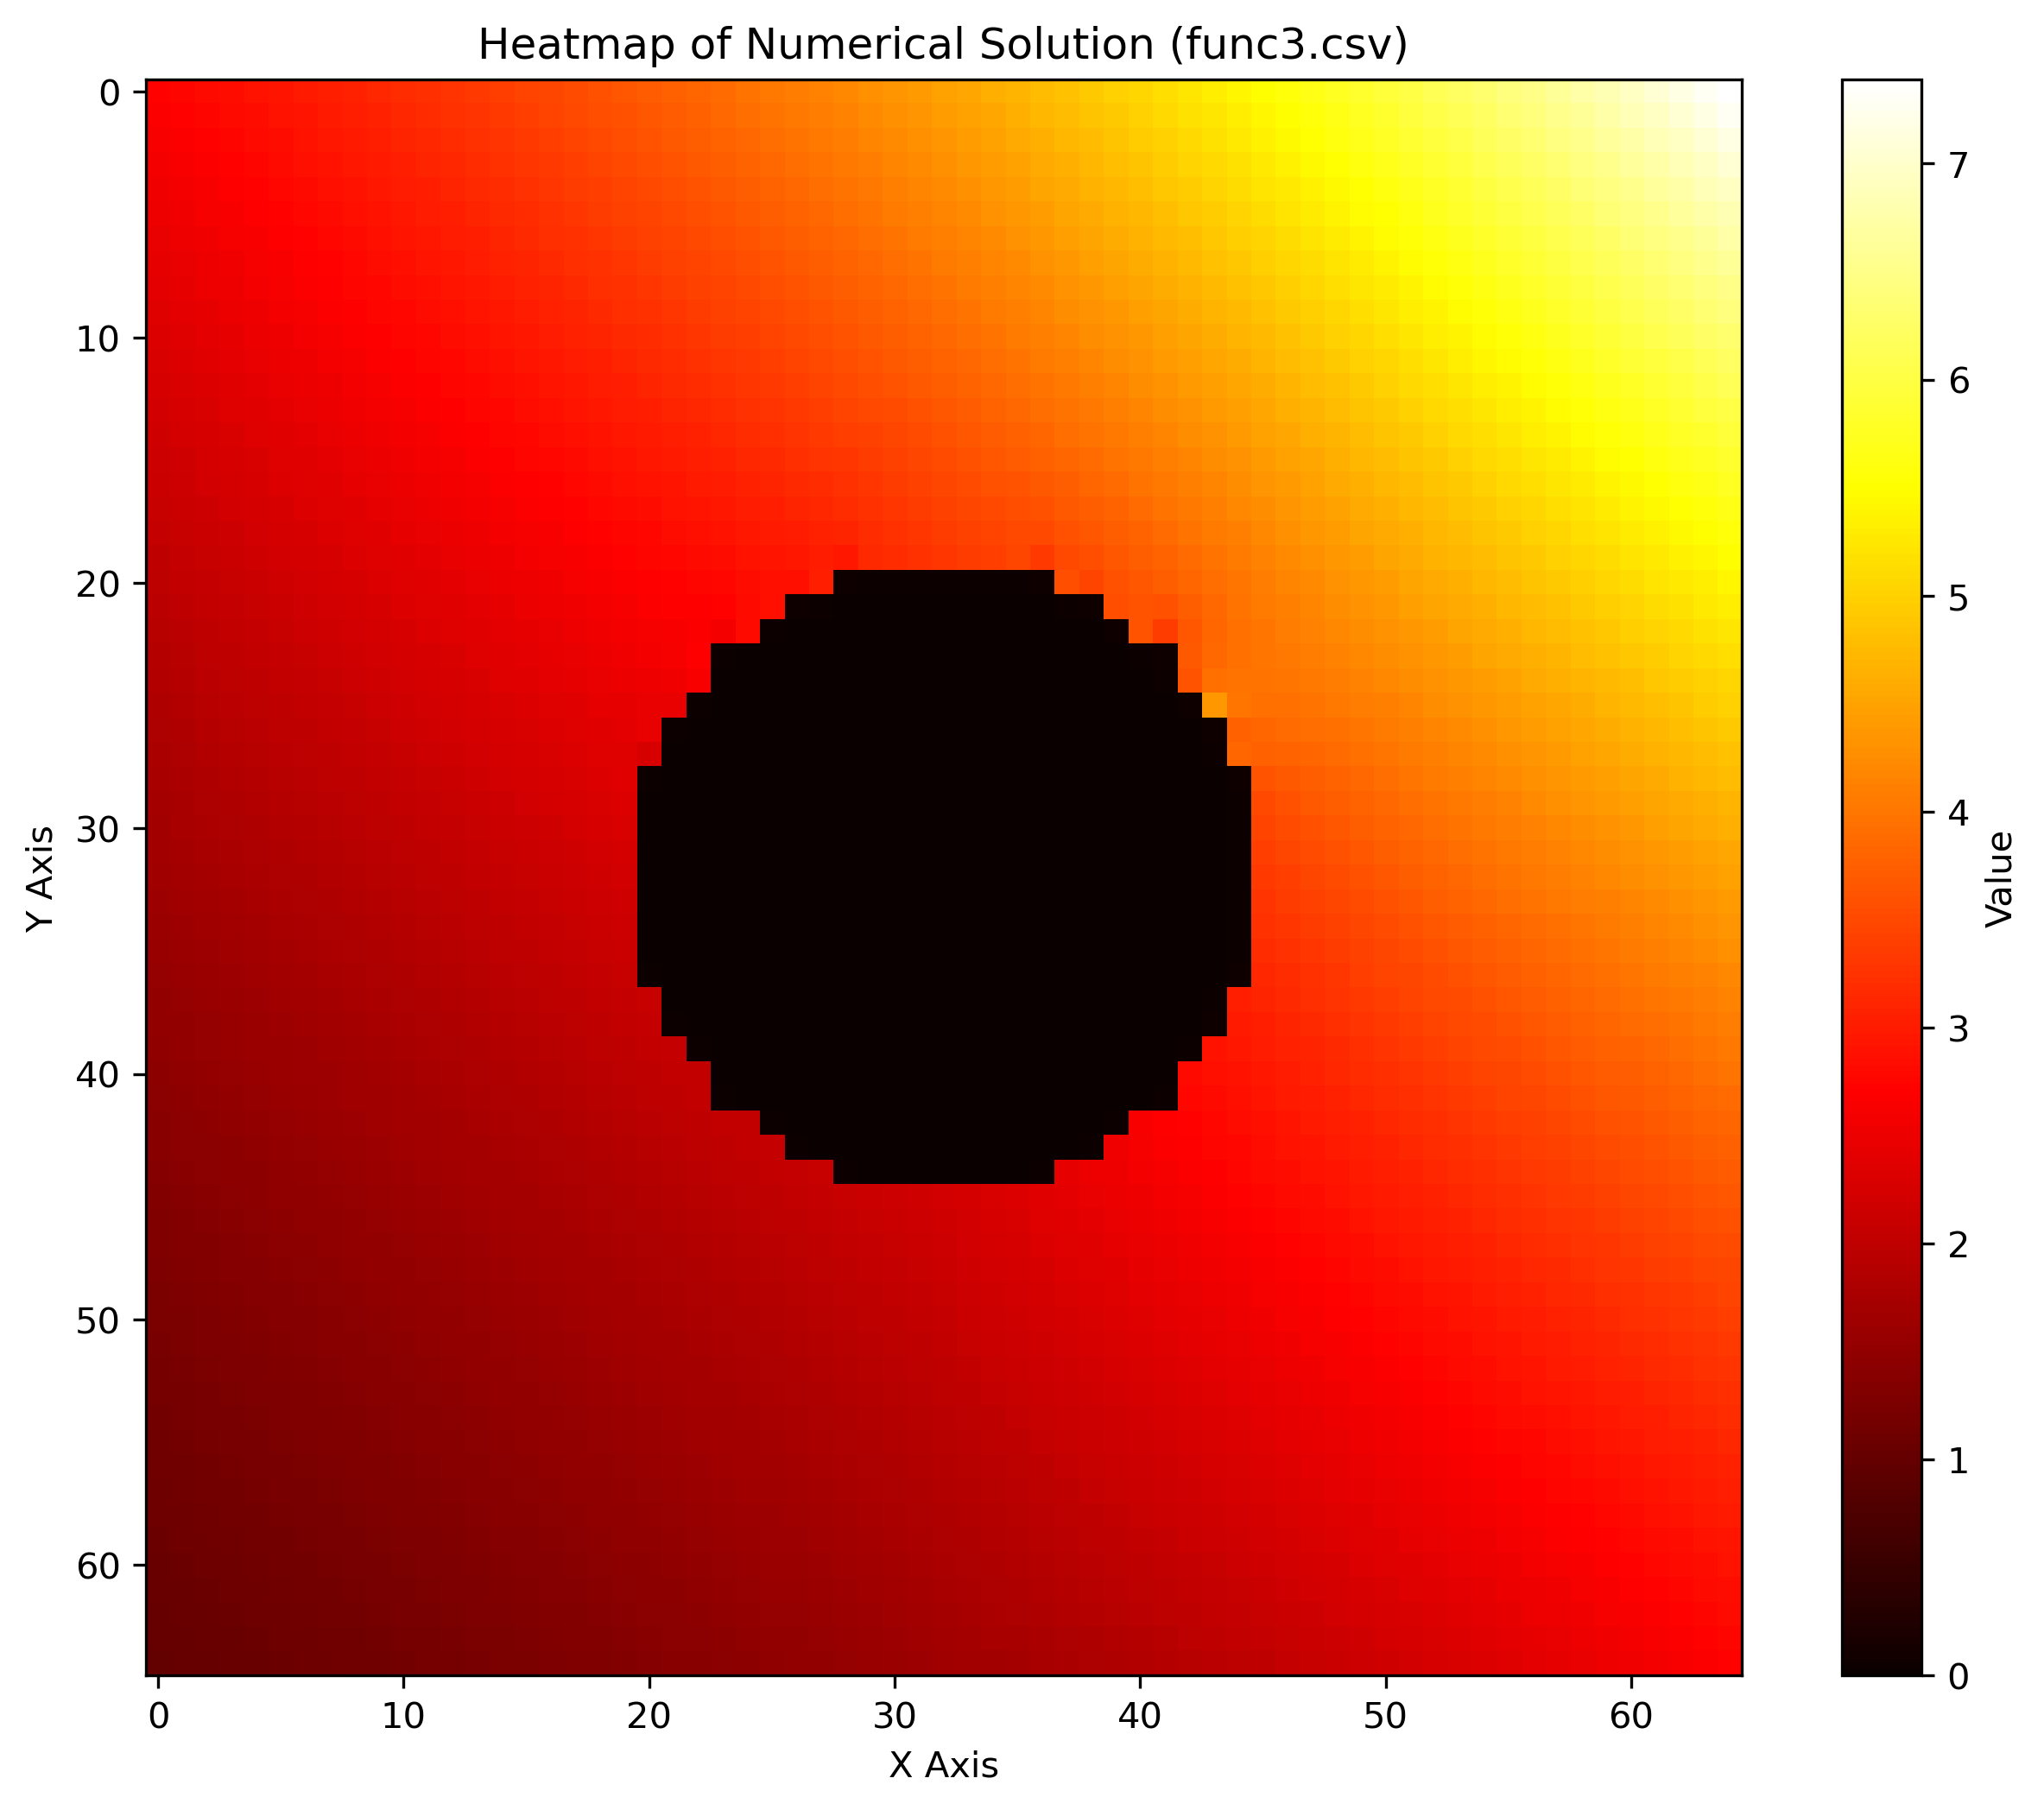
\includegraphics[width=\textwidth]{func3.png}
        \caption{$u = \exp(x + y)$}
        \label{fig:u_exp}
    \end{subfigure}
    \hfill
    \begin{subfigure}[b]{0.35\textwidth}
        \centering
        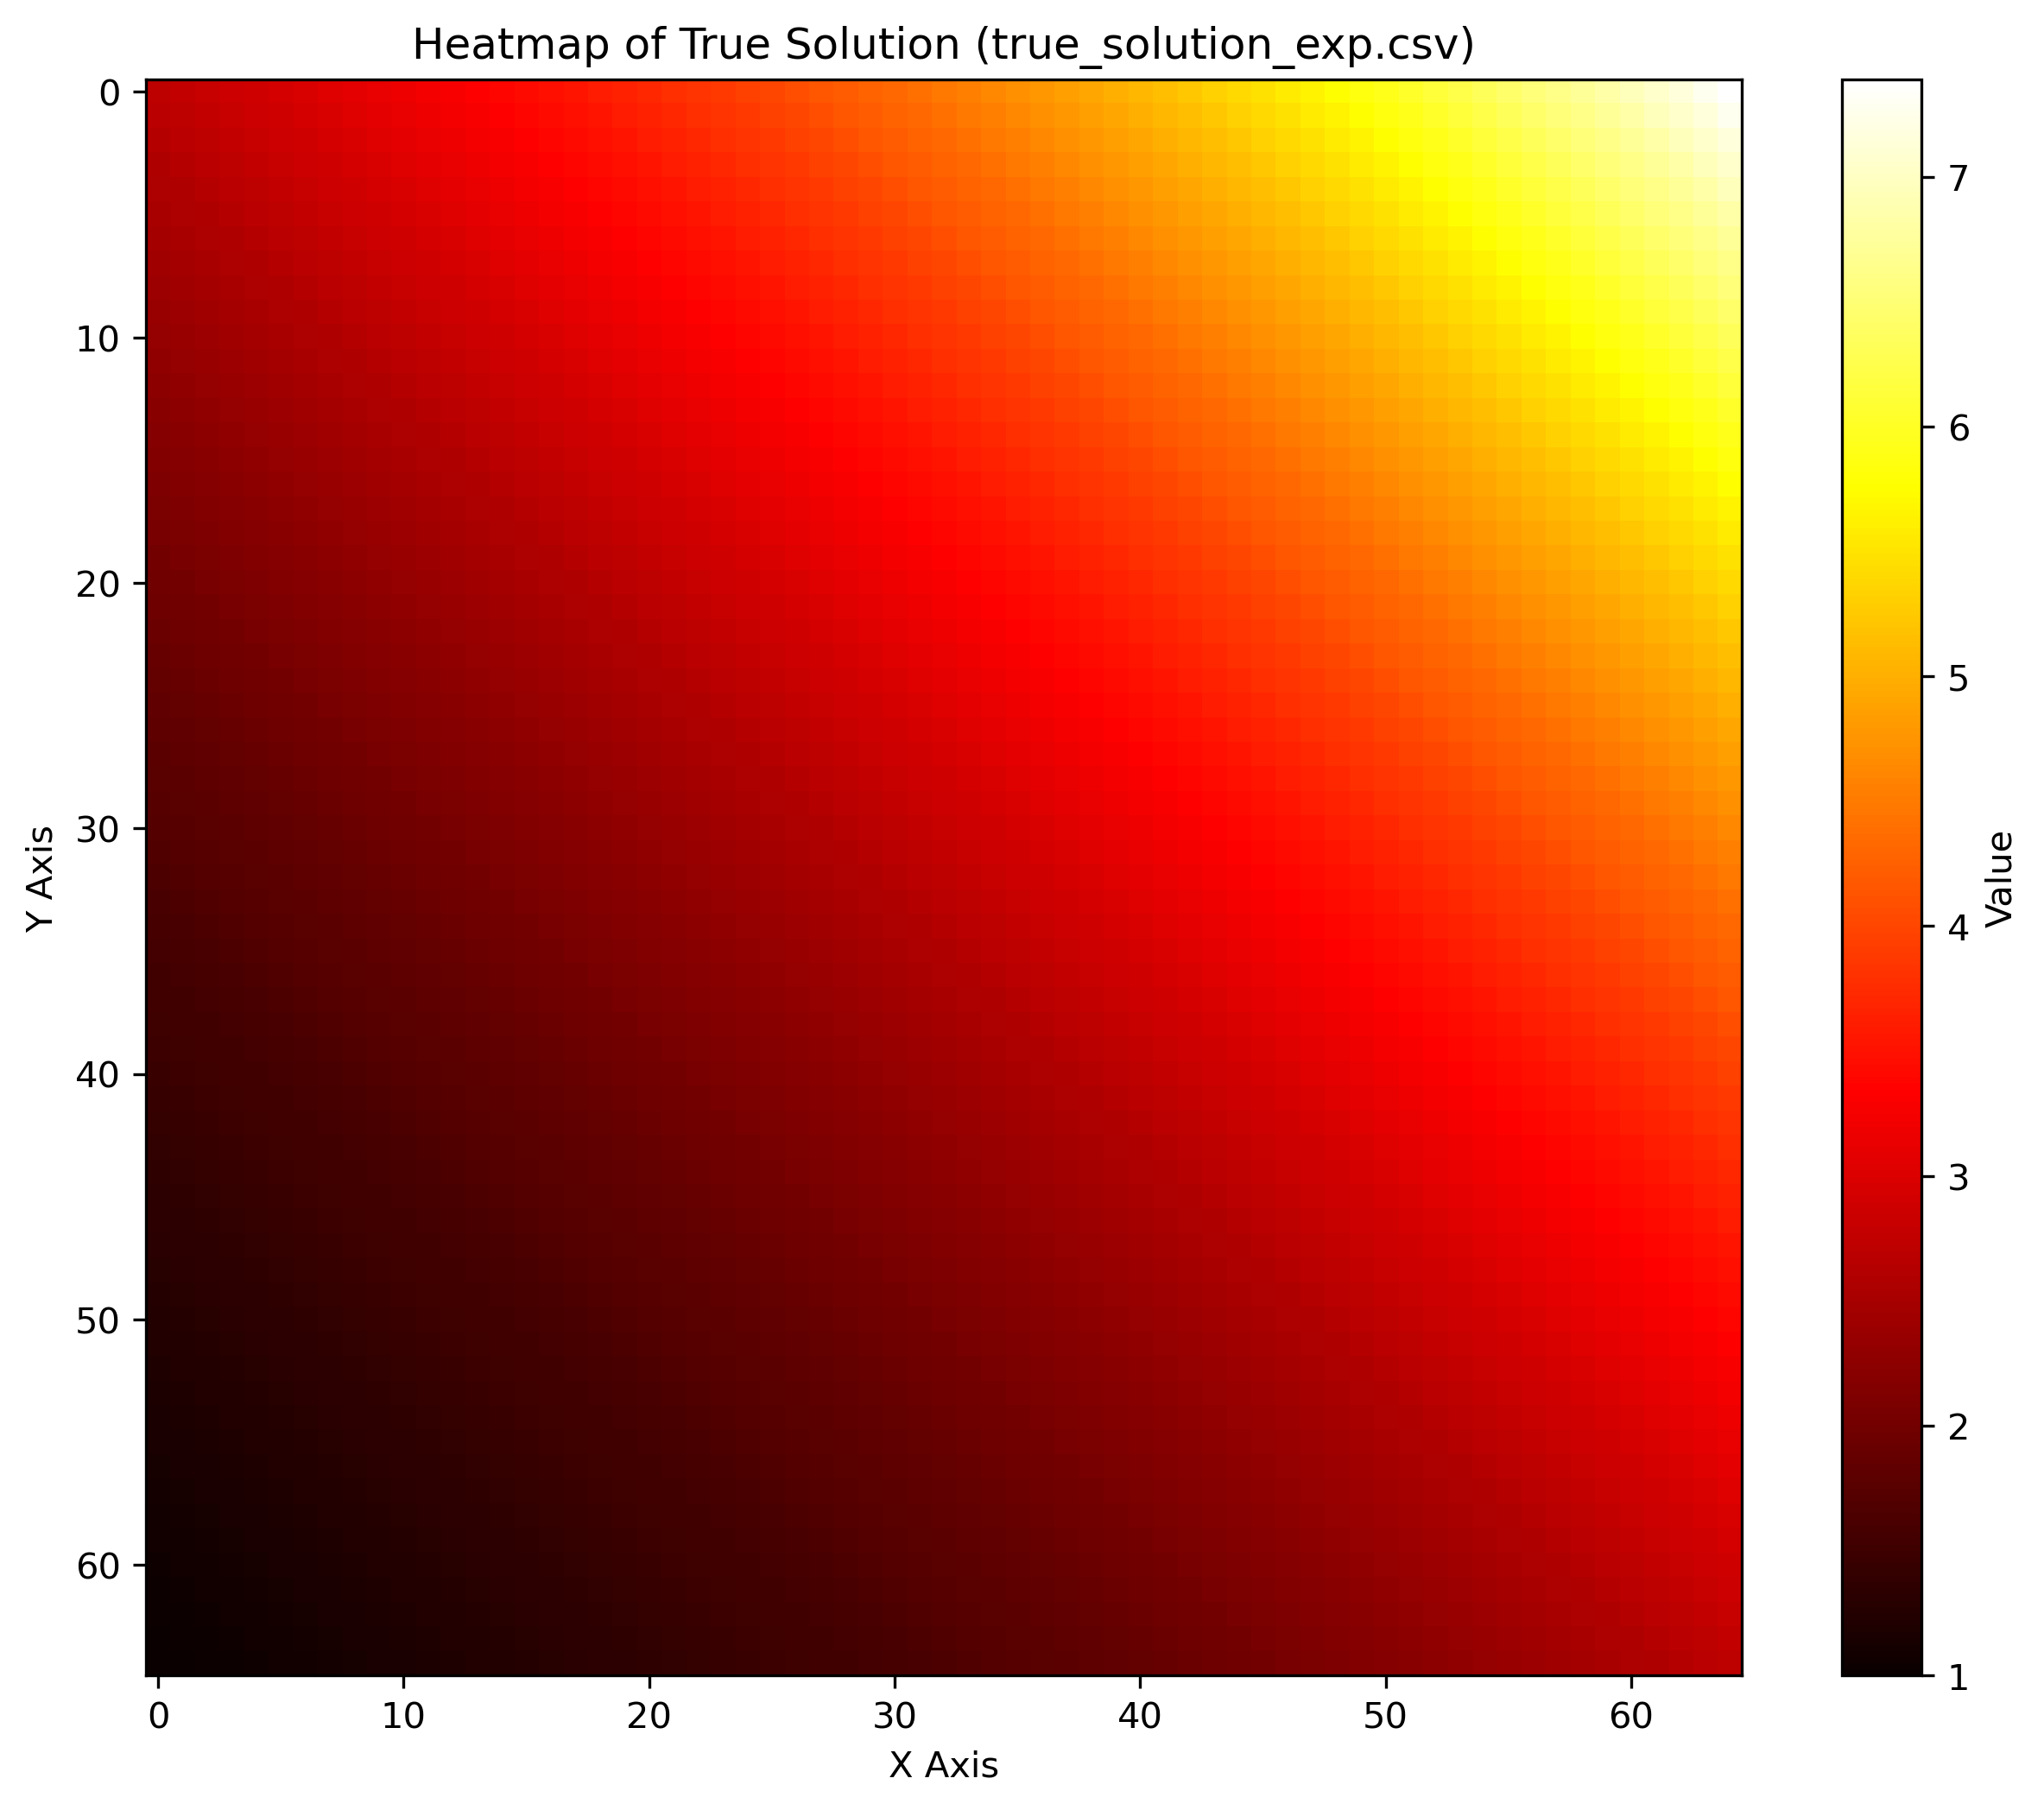
\includegraphics[width=\textwidth]{error_analysis_test/true_solution_exp.png}
        \caption{对应真解}
        \label{fig:true_solution_exp}
    \end{subfigure}
    \caption{效果展示}
    \label{fig:results}
\end{figure}

\end{document}
